% Cashew Network User Manual - Nintendo Wii Style
% Compile with: xelatex cashew-manual.tex (or lualatex for Japanese Unicode support)
% For ASCII-only version, use: pdflatex cashew-manual.tex

\documentclass[11pt,a4paper]{article}

% Packages
\usepackage{ifxetex,ifluatex}
\ifxetex
  % XeLaTeX - supports Unicode natively
  \usepackage{fontspec}
  \usepackage{xeCJK}
  % Set Japanese font (try system default first, fallback to common ones)
  \IfFontExistsTF{MS Gothic}{
    \setCJKmainfont{MS Gothic}
  }{
    \IfFontExistsTF{Noto Sans CJK JP}{
      \setCJKmainfont{Noto Sans CJK JP}
    }{
      % Let system pick default CJK font
    }
  }
\else
  \ifluatex
    % LuaLaTeX - also supports Unicode
    \usepackage{fontspec}
    \usepackage{luatexja-fontspec}
  \else
    % pdfLaTeX - traditional, no Unicode
    \usepackage[utf8]{inputenc}
    \usepackage[T1]{fontenc}
  \fi
\fi

\usepackage{graphicx}
\usepackage{xcolor}
\usepackage{tcolorbox}
\usepackage{fontawesome5}
\usepackage{listings}
\usepackage{hyperref}
\usepackage{geometry}
\usepackage{fancyhdr}
\usepackage{tikz}
\usepackage{soul}

% Page layout
\geometry{margin=1in, top=1.2in, bottom=1.2in}

% Colors (Nintendo Wii inspired - soft, friendly)
\definecolor{cashewbrown}{RGB}{139,69,19}
\definecolor{nutgold}{RGB}{218,165,32}
\definecolor{softblue}{RGB}{135,206,235}
\definecolor{lightgray}{RGB}{245,245,245}
\definecolor{darkgray}{RGB}{64,64,64}
\definecolor{successgreen}{RGB}{76,175,80}

% Header/Footer
\pagestyle{fancy}
\fancyhf{}
\fancyhead[L]{\small\textcolor{cashewbrown}{\textbf{Cashew Network}}}
\fancyhead[R]{\small\textcolor{cashewbrown}{User Manual v0.1.0}}
\fancyfoot[C]{\thepage}
\renewcommand{\headrulewidth}{0.5pt}
\renewcommand{\footrulewidth}{0pt}

% Custom boxes (Wii-style)
\tcbuselibrary{skins}

\newtcolorbox{infobox}[1]{
  colback=softblue!5,
  colframe=softblue!80!black,
  fonttitle=\bfseries,
  title=#1,
  rounded corners,
  attach boxed title to top left={yshift=-2mm, xshift=5mm},
  boxed title style={rounded corners, colback=softblue!80!black}
}

\newtcolorbox{warningbox}{
  colback=nutgold!10,
  colframe=nutgold!80!black,
  fonttitle=\bfseries,
  title=\faExclamationTriangle\ Important,
  rounded corners
}

\newtcolorbox{tipbox}{
  colback=successgreen!10,
  colframe=successgreen!80!black,
  fonttitle=\bfseries,
  title=\faLightbulb\ Pro Tip,
  rounded corners
}

% Code listings
\lstdefinestyle{cashewstyle}{
  backgroundcolor=\color{lightgray},
  commentstyle=\color{darkgray},
  keywordstyle=\color{cashewbrown}\bfseries,
  numberstyle=\tiny\color{darkgray},
  stringstyle=\color{nutgold},
  basicstyle=\ttfamily\small,
  breaklines=true,
  frame=single,
  rulecolor=\color{cashewbrown!50},
  numbers=left,
  tabsize=2,
  showstringspaces=false
}
\lstset{style=cashewstyle}

% Hyperlinks
\hypersetup{
  colorlinks=true,
  linkcolor=cashewbrown,
  urlcolor=softblue,
  pdftitle={Cashew Network User Manual},
  pdfauthor={Cashew Team}
}

% Title page
\title{
  \begin{tikzpicture}[remember picture, overlay]
    \node[anchor=north] at (current page.north) {
      % Cashew logo placeholder
    };
  \end{tikzpicture}
  \vspace{3cm}
  {\Huge\textcolor{cashewbrown}{\textbf{Cashew Network}}}\\[0.5cm]
  {\Large User Manual}\\[0.3cm]
  {\large Freedom over profit. Privacy over surveillance.}
}
\author{
  Version 0.1.0 --- February 2026
}
\date{}

\begin{document}

\maketitle
\newpage

% Welcome message
\begin{center}

\vspace{1cm}

\begin{infobox}{So You Want to Escape Big Tech}
\centering
\textit{``Yeah, we get it. You're tired of corporations owning your data.''}

\vspace{0.5cm}

Welcome to Cashew, where \textbf{you} actually own your stuff,\\
\textbf{you} decide who sees it, and nobody can pull the plug on you.\\
No rent-seeking, no surveillance capitalism, no bullshit.

\vspace{0.3cm}

This manual will show you how it works.\\
Try not to break anything. 
\end{infobox}
\end{center}

\newpage

\tableofcontents
\newpage

% ============================================================================
\section{Getting Started}

\subsection{What is Cashew?}

Cashew is a \textbf{peer-to-peer content distribution network}. Think BitTorrent, but for hosting websites. And you don't have to explain to your ISP why you're seeding \textit{that} torrent.

\begin{center}
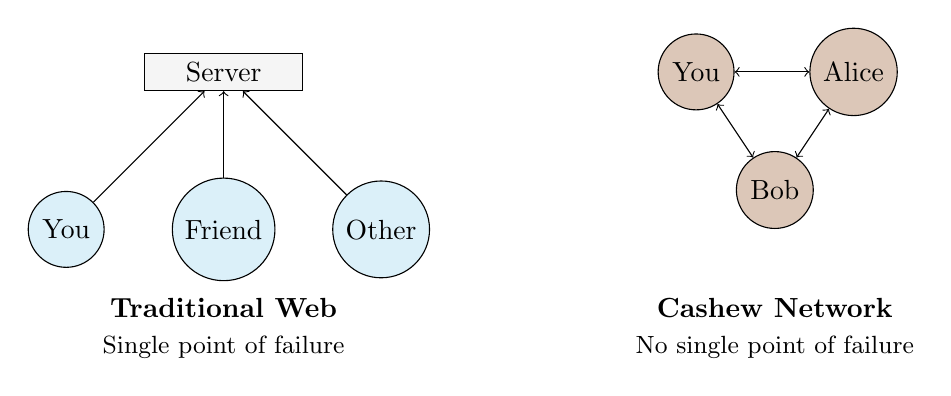
\begin{tikzpicture}
  % Traditional web
  \node[draw, rectangle, fill=lightgray, minimum width=2cm] (server) at (0,3) {Server};
  \node[draw, circle, fill=softblue!30] (user1) at (-2,1) {You};
  \node[draw, circle, fill=softblue!30] (user2) at (0,1) {Friend};
  \node[draw, circle, fill=softblue!30] (user3) at (2,1) {Other};
  
  \draw[->] (user1) -- (server);
  \draw[->] (user2) -- (server);
  \draw[->] (user3) -- (server);
  
  \node at (0,0) {\textbf{Traditional Web}};
  \node at (0,-0.5) {\small Single point of failure};
  
  % Cashew network
  \node[draw, circle, fill=cashewbrown!30] (p1) at (6,3) {You};
  \node[draw, circle, fill=cashewbrown!30] (p2) at (8,3) {Alice};
  \node[draw, circle, fill=cashewbrown!30] (p3) at (7,1.5) {Bob};
  
  \draw[<->] (p1) -- (p2);
  \draw[<->] (p2) -- (p3);
  \draw[<->] (p3) -- (p1);
  
  \node at (7,0) {\textbf{Cashew Network}};
  \node at (7,-0.5) {\small No single point of failure};
\end{tikzpicture}
\end{center}

\begin{tipbox}
If one person goes offline, the content stays up. It's like having multiple copies of the same book scattered across your friend group.
\end{tipbox}

\subsection{Key Features}

\begin{itemize}
  \item[\faCheck] \textbf{You own your data} --- It's on YOUR disk, not Amazon's
  \item[\faCheck] \textbf{Privacy first} --- No tracking pixels, no analytics
  \item[\faCheck] \textbf{Invite-only} --- Your network, your rules
  \item[\faCheck] \textbf{Free forever} --- No VC funding to burn through
  \item[\faCheck] \textbf{Host anything} --- As long as it's legal (we're not your lawyers)
\end{itemize}

% ============================================================================
\section{Installation}

\subsection{System Requirements}

\textit{It's written in C++, so honestly...}

\begin{tabular}{ll}
\textbf{Bare minimum:} & Electricity (and a computer) \\
\textbf{OS:} & Windows, Linux, macOS, or whatever runs C++ \\
\textbf{RAM:} & 512 MB minimum, 2 GB recommended \\
\textbf{Storage:} & 100 MB for program, + your content \\
\textbf{Network:} & Internet connection (for P2P) \\
\end{tabular}

\begin{tipbox}
If your machine can compile and run C++ code, it can run Cashew. We've even heard rumors of it running on a toaster (results pending).
\end{tipbox}

\subsection{Installation on Windows}

\begin{enumerate}
  \item Download MSYS2 from \url{https://www.msys2.org/}
  \item Open MSYS2 UCRT64 terminal
  \item Install dependencies:
  
\begin{lstlisting}[language=bash]
pacman -Syu
pacman -S mingw-w64-ucrt-x86_64-gcc \
          mingw-w64-ucrt-x86_64-cmake \
          mingw-w64-ucrt-x86_64-ninja \
          mingw-w64-ucrt-x86_64-libsodium \
          mingw-w64-ucrt-x86_64-spdlog \
          mingw-w64-ucrt-x86_64-nlohmann-json
\end{lstlisting}

  \item Clone and build Cashew:
  
\begin{lstlisting}[language=bash]
git clone https://github.com/Plutomaster28/cashew.git
cd cashew
cmake -B build -G Ninja -DCMAKE_BUILD_TYPE=Release
ninja -C build
\end{lstlisting}

  \item Run: \texttt{.\textbackslash build\textbackslash src\textbackslash cashew.exe}
\end{enumerate}

\subsection{Installation on Linux}

\begin{lstlisting}[language=bash]
# Ubuntu/Debian
sudo apt update
sudo apt install build-essential cmake ninja-build \
                 libsodium-dev libspdlog-dev nlohmann-json3-dev

# Clone and build
git clone https://github.com/Plutomaster28/cashew.git
cd cashew
cmake -B build -G Ninja -DCMAKE_BUILD_TYPE=Release
ninja -C build

# Run
./build/src/cashew
\end{lstlisting}

% ============================================================================
\section{Quick Start}

\subsection{Starting Your Node}

\begin{infobox}{Let's Get You Running!}
Getting started with Cashew is straightforward:

\begin{enumerate}
  \item Start the Cashew node (stores content)
  \item Start the Perl frontend (optional, for browsers)
  \item Upload and share content
\end{enumerate}

Let's do it!
\end{infobox}

\subsubsection{Step 1: Start the Node}

\begin{lstlisting}[language=bash]
# Windows
.\build\src\cashew.exe

# Linux/macOS
./build/src/cashew
\end{lstlisting}

You should see:

\begin{lstlisting}[language=text, numbers=none]
==========================================
Cashew Network Node v0.1.0
Freedom over profit. Privacy over surveillance.
==========================================

Gateway:    http://localhost:8080
WebSocket:  ws://localhost:8080/ws

Node ID:    2ada83c1819a5372...
Storage:    0 items
Networks:   0

Press Ctrl+C to shutdown
\end{lstlisting}

\textbf{What just happened?}

Your node is now:
\begin{itemize}
  \item Running HTTP gateway on port 8080
  \item Storing content in \texttt{./data/storage/}
  \item Exposing API endpoints (\texttt{/api/status}, \texttt{/api/thing/\{hash\}})
\end{itemize}

Visit \url{http://localhost:8080} to see a basic status page.

\subsubsection{Step 2: Start the Perl Frontend (Optional)}

The Cashew node only provides API access. To let browsers VIEW content nicely, run the Perl frontend:

\begin{lstlisting}[language=bash]
# Install Perl dependencies (MSYS2)
pacman -S mingw-w64-ucrt-x86_64-perl \
          mingw-w64-ucrt-x86_64-perl-cgi

# Go to example directory
cd examples/perl-cgi

# Start Perl server on port 8081
perl server.pl
\end{lstlisting}

Now you have TWO services:
\begin{itemize}
  \item \textbf{Cashew node} (localhost:8080) --- stores content, API
  \item \textbf{Perl gateway} (localhost:8081) --- serves to browsers
\end{itemize}

\subsubsection{Step 3: Upload Content}

\textbf{Easy way:} Use the upload demo:

\begin{lstlisting}[language=bash]
cd examples/perl-full-demo
perl server.pl
# Visit http://localhost:8082 for upload UI
\end{lstlisting}

\textbf{Manual way:} Copy files directly to storage:

\begin{lstlisting}[language=bash]
# Copy your file
cp myfile.html data/storage/content/

# Calculate BLAKE3 hash (becomes Thing ID)
b3sum myfile.html

# Create metadata
echo '{"mime_type":"text/html"}' > \
  data/storage/metadata/{hash}.json

# Access via: /api/thing/{hash}
\end{lstlisting}

\begin{tipbox}
\textbf{Pro Tip:} The Perl upload demo (\texttt{perl-full-demo}) is the easiest way to test uploading files. It gives you a web form and automatically calculates hashes!
\end{tipbox}

% ============================================================================
\section{Creating Content}

\subsection{Understanding ``Things''}

In Cashew, we call any piece of content a \textbf{Thing}. It could be:

\begin{itemize}
  \item A website
  \item A document
  \item An image or photo album
  \item Music files
  \item Videos
  \item Literally \textit{anything}!
\end{itemize}

\subsection{Content Addressing Magic}

\begin{center}
\begin{tcolorbox}[colback=lightgray!30, colframe=cashewbrown, width=0.8\textwidth]
\centering
\textbf{Traditional Web}\\[0.3cm]
\texttt{example.com/page.html}\\
$\downarrow$\\
Server controls it\\
Can change anytime\\
Can disappear\\[0.5cm]

\textbf{Cashew Network}\\[0.3cm]
\texttt{cashew://abc123...}\\
$\downarrow$\\
Content IS the address!\\
Hash never changes\\
Lives forever!
\end{tcolorbox}
\end{center}

\begin{warningbox}
\textbf{Key Insight:} If the hash matches, the content is \textit{exactly} what you asked for. No tampering possible!
\end{warningbox}

% ============================================================================
\section{How Hosting Works}

\subsection{The P2P Architecture}

Cashew uses \textbf{peer-to-peer (P2P) networking} --- there's no central server. When you host content:

\begin{center}
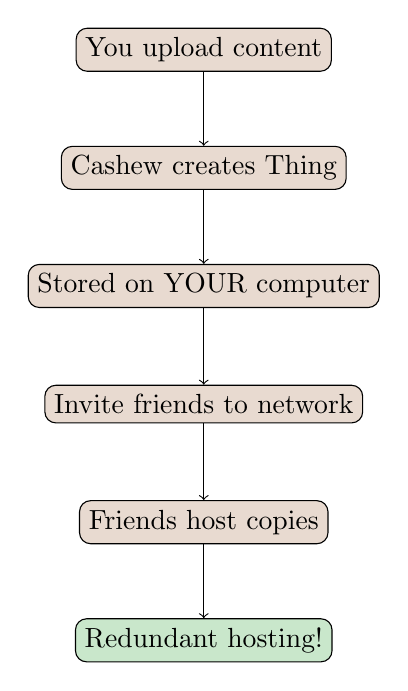
\begin{tikzpicture}[node distance=1.5cm]
  \node[draw, rectangle, rounded corners, fill=cashewbrown!20] (upload) {You upload content};
  \node[draw, rectangle, rounded corners, fill=cashewbrown!20, below of=upload] (thing) {Cashew creates Thing};
  \node[draw, rectangle, rounded corners, fill=cashewbrown!20, below of=thing] (store) {Stored on YOUR computer};
  \node[draw, rectangle, rounded corners, fill=cashewbrown!20, below of=store] (invite) {Invite friends to network};
  \node[draw, rectangle, rounded corners, fill=cashewbrown!20, below of=invite] (replicate) {Friends host copies};
  \node[draw, rectangle, rounded corners, fill=successgreen!30, below of=replicate] (result) {Redundant hosting!};
  
  \draw[->] (upload) -- (thing);
  \draw[->] (thing) -- (store);
  \draw[->] (store) -- (invite);
  \draw[->] (invite) -- (replicate);
  \draw[->] (replicate) -- (result);
\end{tikzpicture}
\end{center}

\subsection{Storage Backend}

\textbf{Where does data live?} Everything is stored in your \texttt{data/} directory:

\begin{lstlisting}[language=bash, numbers=none]
data/
├── storage/
│   ├── content/          # Actual files (by hash)
│   │   ├── abc123...     # Thing content
│   │   ├── def456...     # Another Thing
│   │   └── ...
│   └── metadata/         # Thing metadata (MIME types)
│       ├── abc123.json
│       └── def456.json
├── ledger/               # Append-only event log
│   └── events.db         # SQLite database
└── networks/             # Network membership data
    ├── network1.json
    └── network2.json
\end{lstlisting}

\begin{tipbox}
\textbf{Content Deduplication:} Same content = same hash! If two people upload identical files, they share the same storage.
\end{tipbox}

\subsection{How Content Serving Works}

\textbf{When someone requests a Thing:}

\begin{enumerate}
  \item Gateway receives HTTP request: \texttt{GET /thing/abc123...}
  \item Storage layer checks: ``Do I have this hash?''
  \item If yes: Serve it directly from disk
  \item If no: Ask network members (``Who has abc123...?'')
  \item Download from peer, verify hash, serve to user
  \item Cache locally for next time
\end{enumerate}

\begin{center}

\begin{tikzpicture}
  \node[draw, rectangle] (browser) at (0,3) {Browser};
  \node[draw, rectangle] (node) at (3,3) {Your Node};
  \node[draw, rectangle] (friend) at (6,3) {Friend's Node};
  
  \draw[->] (browser) -- node[above] {\tiny GET /thing/abc123} (node);
  \draw[->] (node) -- node[above] {\tiny "Got abc123?"} (friend);
  \draw[<-] (node) -- node[below] {\tiny sends content} (friend);
  \draw[<-] (browser) -- node[below] {\tiny serves content} (node);
\end{tikzpicture}
\end{center}

\subsection{WebSocket Real-Time Updates}

Cashew uses \textbf{WebSockets} for instant notifications:

\begin{itemize}
  \item New content available
  \item Network member joined/left
  \item Thing updated by network
  \item Reputation changes
\end{itemize}

Connect to: \texttt{ws://localhost:8080/ws}

% ============================================================================
\section{Cryptography \& Key System}

\subsection{Node Identity}

Every Cashew node has a \textbf{unique cryptographic identity}:

\begin{lstlisting}[numbers=none]
Node Identity
├── Private Key (Ed25519)  <- Keep this SECRET!
├── Public Key (Ed25519)   <- Share with friends
└── Node ID (BLAKE3 hash)  <- Your network address
\end{lstlisting}

\textbf{Ed25519 Elliptic Curve Cryptography:}
\begin{itemize}
  \item \textbf{Fast:} Sign/verify in microseconds
  \item \textbf{Small:} 32-byte keys, 64-byte signatures
  \item \textbf{Secure:} 128-bit security level
  \item \textbf{Modern:} Used by Signal, SSH, TLS 1.3
\end{itemize}

\subsection{How Authentication Works}

\textbf{When you join a network:}

\begin{enumerate}
  \item Friend sends you invitation (signed with their key)
  \item You verify signature (proves it's really them)
  \item You accept invitation (sign acceptance with your key)
  \item Network records both signatures (permanent proof)
\end{enumerate}

\begin{lstlisting}[language=JSON, numbers=none]
{
  "network_id": "my-blog",
  "invitee": "your-node-id",
  "role": "full",
  "timestamp": 1738368000,
  "signature": "4a3b9c..."  <- Signed by inviter
}
\end{lstlisting}

\subsection{Content Verification}

Every Thing is \textbf{content-addressed} using \textbf{BLAKE3 hashing}:

\begin{center}
\begin{tcolorbox}[colback=lightgray!30, colframe=cashewbrown, width=0.8\textwidth]
\centering
Original Content $\rightarrow$ BLAKE3 Hash Function $\rightarrow$ Hash (Thing ID)

\vspace{0.3cm}

``Hello, World!'' $\rightarrow$ \texttt{blake3()} $\rightarrow$ \texttt{abc123def456...}
\end{tcolorbox}
\end{center}

\textbf{Why BLAKE3?}
\begin{itemize}
  \item \textbf{Fastest} cryptographic hash (8x faster than SHA-256)
  \item \textbf{Secure:} Collision-resistant, preimage-resistant
  \item \textbf{Parallel:} Uses all CPU cores
  \item \textbf{Verified:} Open-source, peer-reviewed
\end{itemize}

\begin{warningbox}
\textbf{Verification process:}\vspace{0.2cm}

Download content $\rightarrow$ Hash it $\rightarrow$ Compare to Thing ID

\vspace{0.2cm}

Match? \faCheck\ Valid content!\quad Mismatch? \faTimes\ Corrupted or fake!
\end{warningbox}

% ============================================================================
\section{Proof-of-Work \& Reputation}

\subsection{Why Proof-of-Work?}

Cashew uses \textbf{lightweight proof-of-work} to prevent spam and build reputation. \textbf{NOT for cryptocurrency!}

\textbf{Goals:}
\begin{itemize}
  \item Prevent spam (costs CPU time)
  \item Build trust (proves commitment)
  \item Prevent Sybil attacks (can't fake effort)
  \item No money involved (this isn't crypto!)
\end{itemize}

\subsection{How It Works}

\textbf{When you want to:}
\begin{itemize}
  \item Join a network
  \item Publish new content
  \item Invite someone
\end{itemize}

You must solve a \textbf{small computational puzzle}:

\begin{lstlisting}[numbers=none]
Goal: Find a number (nonce) such that:

  BLAKE3(message + nonce) < difficulty_target

Example:
  message = "Join network 'my-blog' as full member"
  nonce = 0, 1, 2, 3, ... (try until valid)
  
  Try nonce=0:     hash = "9a2f..."  X Too high
  Try nonce=1:     hash = "8d4c..."  X Too high  
  Try nonce=2:     hash = "7b1e..."  X Too high
  ...
  Try nonce=1847:  hash = "0003..."  [*] Success!
\end{lstlisting}

\subsection{Difficulty Levels}

\begin{center}
\begin{tabular}{|l|l|l|}
\hline
\textbf{Action} & \textbf{Difficulty} & \textbf{Avg Time} \\ \hline
View content & None & 0 sec \\ \hline
Join network (invited) & Low & $\sim$1 sec \\ \hline
Publish content & Medium & $\sim$5 sec \\ \hline
Create network & High & $\sim$30 sec \\ \hline
Invite member & Medium & $\sim$5 sec \\ \hline
\end{tabular}
\end{center}

\vspace{0.3cm}

\textit{Difficulty = number of leading zero bits required in hash}

\subsection{Reputation System}

Every action you take builds \textbf{reputation}:

\begin{lstlisting}[numbers=none]
Reputation Score
├── Proof-of-Work solved (+points)
├── Content hosted (+points per GB/day)
├── Uptime (+points per hour online)
├── Invitations honored (+points)
└── Bad behavior (-points)
\end{lstlisting}

\textbf{Why reputation matters:}
\begin{itemize}
  \item Higher reputation $\rightarrow$ More trusted
  \item Trusted nodes get priority for network slots
  \item Reputation is network-specific (can't transfer)
  \item Founder always has highest reputation
\end{itemize}

\begin{tipbox}
\textbf{Example reputation calculation:}

\begin{tabular}{ll}
Base: & 0 \\
+ Joined network (PoW solved): & +10 \\
+ Hosted 500MB for 7 days: & +35 \\
+ 99\% uptime this week: & +50 \\
+ Invited 2 members who stayed: & +20 \\
\hline
\textbf{Total:} & \textbf{115 reputation points}
\end{tabular}
\end{tipbox}

\subsection{Spam Prevention}

Combining \textbf{PoW + Reputation} prevents abuse:

\begin{enumerate}
  \item Attacker wants to spam network with fake content
  \item Must solve PoW for each Thing ($\sim$5 sec each)
  \item Reputation starts at 0 (low priority)
  \item Other members can ignore low-reputation nodes
  \item After X rejections, auto-banned
  \item Creating new identity requires PoW
  \item[$\rightarrow$] \textbf{Expensive to create many fake identities!}
\end{enumerate}

% ============================================================================
\section{Hosting with Perl + CGI}

\begin{infobox}{Retro Vibes}
Perl + CGI is like finding your dad's old cassette tapes. Ancient, dusty, but it still works.

Perfect for:
\begin{itemize}
  \item Raspberry Pi hosting
  \item That spare PC from 2009
  \item Pretending it's the 90s again
  \item Actually learning how the web works (without 50 layers of JavaScript frameworks)
\end{itemize}
\end{infobox}

\subsection{Why Perl + CGI?}

\begin{itemize}
  \item[\faCheck] \textbf{Lightweight} --- Runs on anything
  \item[\faCheck] \textbf{No build step} --- Just write and run
  \item[\faCheck] \textbf{Portable} --- Works everywhere
  \item[\faCheck] \textbf{Simple} --- Great for beginners
\end{itemize}

\subsection{Simple CGI Gateway Example}

Create \texttt{cashew-gateway.pl}:

\begin{lstlisting}[language=Perl]
#!/usr/bin/env perl
use strict;
use warnings;
use CGI;
use JSON;
use LWP::UserAgent;

# Configuration
my $CASHEW_API = "http://localhost:8080/api";

# Create CGI object
my $cgi = CGI->new;

# Get the requested path
my $path = $cgi->path_info() || '/';

# Route to appropriate handler
if ($path =~ m{^/thing/([a-f0-9]{64})$}) {
    serve_thing($1);
} elsif ($path eq '/networks') {
    list_networks();
} else {
    show_home();
}

sub serve_thing {
    my ($hash) = @_;
    my $ua = LWP::UserAgent->new;
    my $response = $ua->get("$CASHEW_API/thing/$hash");
    
    if ($response->is_success) {
        print $cgi->header(
            -type => $response->header('Content-Type')
        );
        print $response->decoded_content;
    } else {
        print $cgi->header(-status => '404 Not Found');
        print "<h1>Thing not found</h1>";
    }
}

# ... more handlers ...
\end{lstlisting}

\begin{tipbox}
Make it executable: \texttt{chmod +x cashew-gateway.pl}
\end{tipbox}

% ============================================================================
\section{Troubleshooting}

\subsection{Common Issues}

\begin{tabular}{|p{0.4\textwidth}|p{0.5\textwidth}|}
\hline
\textbf{Problem} & \textbf{Solution} \\ \hline
Port 8080 already in use & Change \texttt{http\_port} in config \\ \hline
Cannot connect to localhost & Check if node is running \\ \hline
Storage directory not writable & Run: \texttt{chmod -R 755 ./data} \\ \hline
Node crashes on startup & Known issue, workaround active \\ \hline
\end{tabular}

\subsection{Getting Help}

\begin{itemize}
  \item[\faGithub] Report issues: \url{https://github.com/Plutomaster28/cashew/issues}
\end{itemize}

% ============================================================================
\section{FAQ}

\textbf{Q: Is Cashew a cryptocurrency?}\\
A: No. If we wanted to make a ponzi scheme we'd be working at a VC firm.

\vspace{0.3cm}

\textbf{Q: Do I need to be online 24/7?}\\
A: Only if you want to be the sole host. Otherwise, convince your friends to help share the load.

\vspace{0.3cm}

\textbf{Q: How much disk space do I need?}\\
A: As much as you're hosting. This isn't the cloud — it's YOUR disk.

\vspace{0.3cm}

\textbf{Q: Is my data encrypted?}\\
A: Content is stored as-is. Want encryption? Do it yourself before uploading.

% ============================================================================
\section{Next Steps}

Congrats, you made it through the manual.

\begin{center}
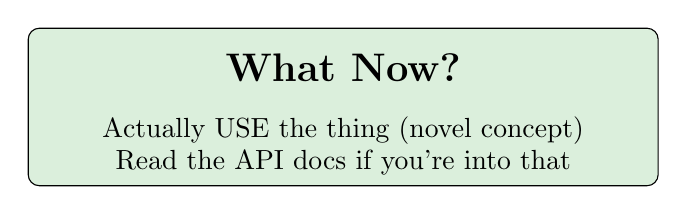
\begin{tikzpicture}
  \node[draw, rectangle, rounded corners, fill=successgreen!20, minimum width=8cm, minimum height=2cm] (box) at (0,0) {};
  \node at (0,0.5) {\Large\textbf{What Now?}};
  \node at (0,-0.3) {Actually USE the thing (novel concept)};
  \node at (0,-0.7) {Read the API docs if you're into that};
\end{tikzpicture}
\end{center}

% ============================================================================
\section{Credits}

\begin{center}

\vspace{1cm}

\textit{``Thanks for actually reading this thing.''}

\textit{``Now go build something cool.''}

\vspace{0.5cm}

Cashew Network was created with love by people who believe\\
the Internet should belong to everyone, not corporations.

\vspace{0.3cm}

\textbf{Made with care and dedication}

\vspace{0.5cm}

\textit{``Freedom over profit. Privacy over surveillance.''}
\end{center}

\vfill

\begin{center}
\small
\textbf{License:} MIT (Free as in freedom!)\\
\textbf{Version:} 0.1.0 --- February 24, 2026
\end{center}

\end{document}

